\chapter{Fundamentação Teórica}
\label{ch:fundamentacao}
\par Neste capítulo ser\~ao fundamentados os conhecimentos b\'asicos para o entendimento do trabalho.

\section{Deficiência} % Este título está completamente problemático....

De acordo com o censo do IBGE, realizado em 2010, cerca de 6.2\% da população brasileira possui algum tipo de deficiência. E a necessidade de inclusão destas pessoas na sociedade é extremamente importante. Do grupo citado anteriormente, cerca de 1.3\% tem algum tipo de deficiência auditiva, e 1.1\% tem deficiências auditivas

Para aqueles com deficiência auditiva, a comunicação e inclusão pode ser feita através da Linguagem Brasileira de Sinais, segunda língua oficial do Brasil desde 2005. Mas, pode-se encontrar problemas com a comunicação através de LIBRAS principalmente pelo fato de, boa parte dos ouvintes não falar esta língua o que acarreta também na baixa utilização desta em diversos meios de comunicação. Um ponto importante apontado no documentário feito pela TVE RS, é que, pessoas com deficiência auditiva, normalmente são alfabetizadas somente com LIBRAS, por terem muita difículdade e falta de estrutura para o aprendizado da Língua Portuguesa. Ainda de acordo com o documentário, para as pessoas com deficiências motoras há os recursos de tecnologias assitivas, que aumentar a facilidade do acesso destas pessoas aos meios sociais, principalmente os digitais.

% Precisa ficar realizando definições de cada uma das deficiências que serão tratadas no trabalho ?? Pensando hoje, acho que deveria sim! 
%% Caso precise, qual o nível de profundidade necessário ? ? ? Não tão profundo, mas a ponto de demonstrar a qual público o trabalho é destinado

\section{Tecnologias assistivas}

% NTAAI -> Verificar como citar esta fonte ! ! !
% Verificar se devo citar tecnologias assistivas, ou no meu caso, recursos assistivos ! ! !
Uma das formas de realizar a inclusão social de pessoas com deficiência é através da inclusão digital, utilizando técnologias assitivas, estes que visam ampliar as habilidades presentes no indivíduo, não o forçando a ter características específicas para a inclusão (NTAAI, 2016). As tecnologias assitivas, de acordo com o Núcleo de Tecnologia Assistiva, Acessibilidade e Inovação da Universidade de Brasilia, podem ser divididas em dois grupos, os recursos, que representam equipamentos que expandem as habilidades dos indivíduos com deficiência, e os serviços, que normalmente são aqueles relacionados a facilitação e capacitação para o uso correto dos recursos assistivos.

% Adicionar dados aqui que fazem jus ao que estou dizendo ! ! !
% Paragrafo abaixo deve antes ser reescrito para o novo escodo do trabalho
% Para aqueles que possuem deficiência motora, a inclusão digital vem através de \textit{mouses} adaptados, formas diferentes de utilizar teclados, ou até mesmo a utilização do computador por comandos de voz. E para os surdos ferramentas que ajudam no processo de interação já levando em consideração problemas com a alfabetização.


%%%%%%%%%%%%%%%%%%% Temporário (Coloquei aqui pois utilizo no trabalho, mas vou falar com o Giuliano)
% \section{Regressões}
% \par Um pequeno descritivo sobre regressões
%%%%%%%%%%%%%%%%%%%

%%% 17/02/2019
% Verificar o que pode ser feito com a análise de regressão
% Vendo o que o Felipinho disse, realmente parece que a regressão está foram do lugar aqui
%%%
% \section{Análise de Regressão} % Ou Regressão linear

% MACHADO -> https://www.ime.usp.br/~fmachado/MAE229/AULA10.pdf
% PETERNELLI -> http://www.dpi.ufv.br/~peternelli/inf162.www.16032004/materiais/CAPITULO9.pdf
%A análise de regressão estuda a relação entre uma variável dependente e outras independentes (MACHADO, 2015). Esta relação é representada através de um modelo matemático (MACHADO, 2015), este que pode ter diferentes formas sendo linear, quadrático, exponencial entre outros (PETERNELLI, 2003). 

% ToDo: Colocar um exemplo ? Se for colocar, qual será ? (02/02/2019)

%%%%%%%%%%%%%
% Antiga definição utilizada: Análise de regressão consiste na aplição de uma análise estatística com o objetivo de verificar a relação entre duas variáveis (PETERNELLI, 2003).
% Aqui eu posso colocar assim: Neste trabalho, após a verificação dos dados fez-se a utilização de regressões lineares
% Claro que isto deverá ser reescrito, até porque coloquei com as minhas palavras
% \par Os métodos de regressão são aqueles que buscam através de variáveis continuas ou categóricas estimar uma outra variável, podendo esta também ser continua ou categórica. Para este trabalho utilizou-se do método de regressão linear, este que básicamente busca através de uma função f(x) mapear a relação de duas variáveis linearmente separáveis.
%%%%%%%%%%%%%

% \section{Correlação de imagens digitais}

% http://www.dpi.inpe.br/~carlos/Academicos/Cursos/Pdi/pdi_estatisticas.html
% Se tudo funcionar da forma que estou pensando, vou colocar este conceito aqui (02/02/2019)
% Pois bem, não funcionou como eu esperada, assim vou manter este conceito de fora do documento (03/02/2019)

% \par A correlação é A, porém para este trabalho ela foi empregada em Imagens digitais

% \subsection{Regressão logistica}

% \par Uma função que divide o espaço, porém levando em consideração variáveis dependentes categóricas
%%%%%%%%%%%%%%%%%%%

\section{Inteligência artificial}

%%%%%%%%%%%%%%%%%%%%% Verificar a necessidade de escrever sobre inteligência artificial ! ! ! No momento (01/02/2019) eu acho que devo escrever sobre

% Rever todas as referências - Provavelmente reescrever o texto nas férias ! ! ! (Já arrumei melhor as coisas neste capítulo (01/02/2019)
% Von Zuben: ftp://ftp.dca.fee.unicamp.br/pub/docs/vonzuben/ea072_2s13/introducao_EA072_2s2013.pdf
% (Winston, 1992) Livro do Winston

Sistemas inteligentes de forma geral são aqueles que apresentam a capacidade de planejar e resolver problemas através de dedução e indução utilizando conhecimentos de situações anteriores \cite{VonZuben2013}, e a inteligência artificial, é um campo da ciência e engenharia de computação \cite{VonZuben2013}, que possibilitam a sistemas computacionais, perceber, raciocionar e agir \cite{Winston1992}.

% Augusto -> http://dcm.ffclrp.usp.br/~augusto/teaching/ami/AM-I-Conceitos-Definicoes.pdf
As técnicas computacionais mais utilizadas para o desenvolvimento e aplicação de inteligência artificial, são aquelas relacionadas ao aprendizado de máquina. Esta que é uma área que tem como objetivo principal, desenvolver técnicas que permitam aos sistemas adquirir conhecimento de forma automática e com estes conhecimentos tomar decisões \cite{Augusto2007}.

% NG -> Curso do andrew
Para a realização do aprendizado de máquina, existem diversas técnicas, que vão de simples regressões estatísticas, até modelos complexos, como às redes neurais artificiais (RNA) (NG, 2016).
%%%%%%%%%%%%%%%%%%%%%

\section{Redes neurais artificiais}

% Colocar mais referências em redes neurais artificiais, exemplos de uso.... acho que fica legal
% Haikin (2001) -> Livro (Redes Neurais: Princípios e Prática)
% Cintra -> Minicurso do INPE (2015)

% É um começo, mas ainda não estou feliz com o resultado.... (01/02/2019)
Redes neurais artificiais são sistemas computacionais que busca modelar o sistema cerebral natural humano, estas que são uma das formas de soluções de problemas apresentados dentro do âmbito de inteligência computacional \cite{Cintra2019}.

%% Não creio que isto esteja escrito da melhor forma, mas está melhor que o texto inicial (01/02/2019)
Por buscar modelar o cérebro humano, as RNAs utilizam como unidade básica de processamento, os neurônios artificiais \cite{Haykin2001}, da mesma forma que o cérebro utiliza os neurônios biológicos. % Preciso criar um complemento para ir para o próximo capítulo ? (01/02/2019)

%Acho que esta segunda parte não está combinando com o resto do texto, mas por agora vou manter aqui
% Por buscar modelar o cérebro humano, a unidade básica de processamento das RNAs são os neurônios (HAYKIN, 2001), estruturas estas que tem fortes ligações com o sistema biológico.

%%%%%%% Partes antigos
% Redes neurais artificiais (RNA) são modelos criados para representar a maneira como o cérebro realiza suas tarefas, sendo estas maciçamente paralelas e distribuidas (HAYKIN, 2001). Ainda de acordo com Haykin (2001), estes modelos para ter bons desempenhos são representados normalmente através de interligações maciças de células computacionais simples, denominadas de neurônios. 
% Veja que, para a criação destes modelos, há uma grande inspiração em aspectos e funcionamentos do cérebro humano (CINTRA, 2015)
% Acho que isto aqui deve ser complementado ! ! ! Com toda a certeza!
% Cintra - Minicurso INPE (2015)
% Como descrito na seção anterior, uma das áreas de aplicação do aprendizado de máquina mais avançadas atualmente são as RNA, que imitam principalmente aspectos do funcionamento do corpo humano, neste caso, o cérebro e suas redes neuronais (CINTRA, 2015). 
%%%%%%%

\subsection{Neurônio biológico}

% Falar sobre sinapses ! ! ! -> Já falei sobre isto ! ! !
% Falar sobre como aprendemos ! ! ! -> Será  mesmo necessário ? ? ?

% Nunes -> Livro
Todo o processamento de informações no cérebro humano, é feito através de elementos biológicos de processamento, que operam em paralelo para a produção de ações apropriadas para cada estímulo recebido pelo corpo. A célula base do sistema nervoso cerebral é o neurônio (Figura \ref{figure:bioneuron}), e sua principal função é conduzir impulsos (Representando os estímulos) levando em consideração as condições do corpo e assim produzindo ações. Os neurônios também são os responsáveis pelos atos do pensamento e armazenamento de informações \cite{livroNunes2016}.

Os neurônios podem ser divididos em três partes elementares, os dendritos, que captam de forma continua os impulsos vindos de outros neurônios, o corpo celular, que processa todas as informações captadas e os axônios que enviam as informações processadas no corpo celular para outros neurônios.

% https://www.researchgate.net/figure/Figura-24-Ilustrativo-de-um-neuronio-biologico_fig17_303369695
\image{1.4}{neuronio-biologico.png}{Ilustração do neurônio biológico}{figure:bioneuron}{\citeonline{Remes2016}}

% SHEPERD -> Artigo
% XAVIER -> Artigo (Divulgado no Alô Ciência) !
% Consultar o livro do Hebb apenas para ter uma certeza!
Estima-se que a rede neural cerebral, possui cerca de 100 bilhões de neurônios, cada um destes mantendo conexão com uma média de 6.000 outros neurônios, gerando cerca de 600 trilhões de conexões (SHEPHERD, 1990). A região de conexão entre os neurônios são chamadas de sinapses, estas que como apresentado por Donald Hebb em 1949, em seu livro \textit{The Organization of Behavior} são fortalecidas todas as vezes em que são utilizadas.

% A regiã entre os neurônios são chamados de sinapses, estas que como apresentado por Donald Hebb em 1949, em seu livro \textit{The Organization of Behavior} tem os caminhos fortalecidos toda vez que é utilizado
% , assim, pode-se entender que, neurônios tem propensões para certas atividades, quando os neurônios utilizados por esta tem suas sinapses bem fortalecidas (XAVIER, 2017).

A Figura \ref{figure:nncotex} demonstra um exemplo de uma pequena parte das redes neuronais responsáveis pelo córtex auditivo.

% ToDo
% https://pt.wikipedia.org/wiki/Ficheiro:Cajal_actx_inter.jpg
% MAnter wikipédia é foda...
\image{0.35}{nn_cortex.jpg}{Rede neural do córtex auditivo}{figure:nncotex}{}

%%% Validar as informações abaixo
% Citar assim Hodgkin e Huxley (1952) ou (Hodgkin; Huxley, 1952) ? ? ?

% McCulloch -> Artigo
% (HODGKIn, HUXLEY, 1952) ? ? ? 
A representação inicial deste conjunto de neurônios em sistemas de computação foram implementadas através de circuitos eletrônicos, com apresentado por McCulloc e Pitts (1943), estes que foram utilizados como base para a criação dos modelos de neurônios artificiais apresentados por Hodgkin e Huxley (1952).
%%%

\subsection{Neurônio artificial}

Como citado anteriormente, os neurônios artificiais, são modelos computacionais para a representação do neurônio biológico nas RNAs, e da mesma forma que em um neurônio biológico, a representação deste é feita com três elementos básicos \cite{Haykin2001}:  

\begin{itemize}
	% Posso colocar Conjunto de sinapses, representado por Xn... ? (02/02/2019)
	\item Conjunto de sinapses, cada uma caracterizada por um peso, este que indica a relevância de cada valor de entrada;
	\item Somador, ou combinador linear, que faz a ponderação dos valores de entrada com as respectivas sinapses do neurônio;
	\item Função de ativação utilizada para restringir os valores de saída do neurônio.
\end{itemize}

Ainda de acordo com \citeonline{Haykin2001}, a estes modelos neuronais pode-se aplicar um \textit{bias}, este que será o responsável pelo aumento ou diminuição dos valores de entrada da função de ativação. Em termos matemáticos, pode-se descrever um neurônio k (Figura \ref{figure:nn_mcculloch}) com as seguintes equações \cite{Haykin2001}:

\begin{equation}
	u_{k} = \sum_{j=1}^{n} w_{kj} x_{j}
\end{equation}
e
\begin{equation}
	y_{k} = f(u_{k} + b_{k})	
\end{equation}
onde $ x_{1}, x_{2}, ..., x_{n} $ são os sinais de entrada; $ w_{k1}, w_{k2}, ..., w_{kn} $ são os pesos sinápticos do neurônio k; $ u_{k} $ é a saída do combinador linear; $ b_{k} $ é o \textit{bias}; $ f(u_{k} + b_{k}) $ a função de ativação; e $ y_{k} $ representa a saída do neurônio.

% Os neurônios artificias, que são modelos de representações dos neurônios biológicos compoem a RNA. O principal modelo de neurônio artificial utilizado, mesmo em arquiteturas mais atuais, é o proposto por McCulloch e Pitts em 1943 (Figura 3). Neste há componentes que fazem referência direta ao neurônio biológico visto anteriormente.

% Imagem adaptada de Haykin (2001)
% \image{0.1}{nn_mculloch.jpg}{Modelo de Neurônio artificial}{figure:nn_mcculloch}{Adaptado de \cite{Haykin2001}}
\begin{figure}[H]
    \centering
   \begin{tikzpicture}[
init/.style={
  draw,
  circle,
  inner sep=2pt,
  font=\Huge,
  join = by -latex
},
init2/.style={
  draw,
  circle,
  inner sep=2pt
},
neuron missing/.style={
    draw=none, 
    scale=4,
    text height=0.333cm,
    execute at begin node=\color{black}$\vdots$
  },
squa/.style={
  draw,
  inner sep=2pt,
  font=\Large,
  join = by -latex
},
squa2/.style={
  draw,
  inner sep=2pt,
  font=\Large
},
start chain=2,node distance=13mm
]
\node[on chain=2] 
  (x2) {$x_2$};
%\node[below of=x2] (dots) {$\vdots$} -- (dots) node[right of=dots] (ldots) {$\vdots$};
%\node[below of=2] (dots) {$\vdots$} -- (dots) node[left of=dots] (ldots) {$\vdots$};
\node[on chain=2,init2,join=by o-latex] 
  {$w_{k2}$};
\node[on chain=2,init] (sigma)
  {$\displaystyle\Sigma$};
\node[on chain=2,squa2,label=above:{\parbox{2cm}{\centering Função de \\ ativação}}](te) {$f$};
\node[on chain=2,label=above:Saída] (sa)
  {$y_k$};
\begin{scope}[start chain=1]
\node[on chain=1] at (0,1.5cm) 
  (x1) {$x_1$};
\node[on chain=1,init2,join=by o-latex] 
  (w1) {$w_{k1}$};
\end{scope}
\begin{scope}[start chain=3]
\node[on chain=3] at (0,-1.5cm) 
  (x3) {$x_n$};
\node[on chain=3, init2,label=below:{\parbox{2cm}{\centering Pesos \\ sinápticos}},join=by o-latex] 
  (w3) {$w_{kn}$};
\end{scope}
\node[label=above:\parbox{2cm}{\centering Bias \\ $b$}] at (sigma|-w1) (b) {};

\draw[-latex] (w1) -- (sigma);
\draw[-latex] (w3) -- (sigma);
\draw[o-latex] (b) -- (sigma);
\draw[-latex] (sigma) -- (te) node[midway,sloped, above]{$v_k$};
\draw[-latex] (te) -- (sa) node[midway,sloped, above]{};
\draw[decorate,decoration={brace,mirror}] (x1.north west) -- node[left=10pt] {Entradas} (x3.south west);
\end{tikzpicture}
    \caption{Neurônio Artificial}
    \fonte{Adaptado de \citeonline{Haykin2001}}
    \label{fig:modelo_neuronio}
\end{figure}

A partir da Figura 3 é possível realizar uma comparação entre cada um dos elementos do neurônio artificial e biológico. Os sinais de entrada, advindos do meio externo, normalmente uma aplicação, são análogos aos impulsos elétricos captados pelos dendritos no neurônio biológico.  Os pesos sinápticos representam a importância do sinal recebido para o neurônio, o que representa as ponderações exercidas pelas junções sinápticas do modelo biológico, ou seja, a força do caminho entre as sinapses, citados anteriormente. O campo de somatório junto a função de ativação, representam o corpo celular do neurônio biológico, é nesta parte que os resultados criados pelo neurônio são calculados \cite{livroNunes2016} 

\subsection{Arquiteturas de rede} 

Para \citeonline{livroNunes2016} uma RNA pode ser constituída de até três partes diferentes, estas denominadas de camadas, as quais são nomeadas a seguir:

\begin{itemize}
    \item Camada de entrada: É a camada responsável pelo recebimento de dados;
    \item Camadas escondidas, intermediárias ou ocultas: São camadas compostas de neurônios responsáveis pela extração de características associadas ao processo ou sistema;
    \item Camadas de saída: Também constituída de neurônios, esta camada é responsável pela produção e apresentação dos resultados finais da rede.
\end{itemize}

Das camadas descritas acima, devem estar presentes em uma RNA no mínimo a camada de entrada e a camada de saída \cite{Cintra2019}.

Diferentes formas de organização de cada uma destas camadas, especialmente relacionadas a forma de relação entre os neurônios, definem as arquiteturas de RNA \cite{livroNunes2016}. \citeonline{Haykin2001} define a existência de duas classes de arquiteturas fundamentais, sendo elas: Redes de alimentação direta, com uma ou várias camadas e Redes recorrentes.

As redes de alimentação direta, são denominadas desta forma por conta de seu fluxo percorrer uma única direção \cite{Cintra2019}, iniciando o fluxo na camada de entrada seguindo pelas diferentes camadas até o neurônio de saída. Este tipo de rede pode possuir uma ou várias camadas ocultas.

% Verificar se devo abreviar a sigla de redes de alimentação direta.... (04/03/2019)
Para as redes de alimentação direta com uma única camada, tem-se como tipo comum a \textit{Perceptron} (Figura \ref{figure:camadaunida}). Em sua estrutura são apresentadas duas camadas, entrada e saída, porém são nomeadas de camada única já que existem operações matemáticas ocorrendo apenas na camada de saída \cite{livroNunes2016}.

\begin{figure}[H]
    \centering
    \def\layersep{2.5cm}
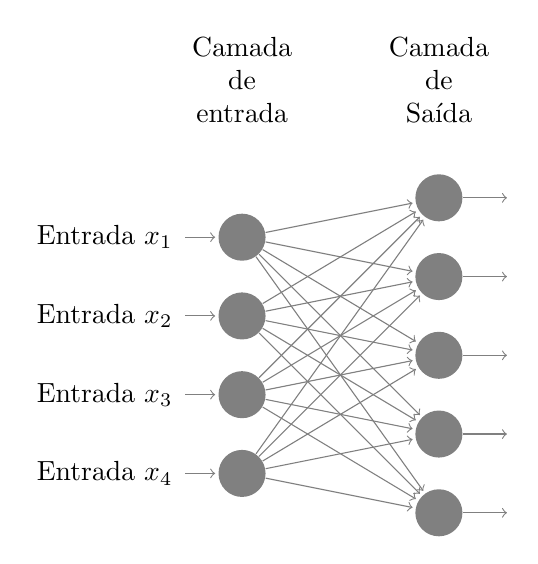
\begin{tikzpicture}[shorten >=1pt,->,draw=black!50, node distance=\layersep]
    \tikzstyle{every pin edge}=[<-,shorten <=1pt]
    \tikzstyle{neuron}=[circle,fill=black!25,minimum size=17pt,inner sep=0pt]
    \tikzstyle{input neuron}=[neuron, fill=black!50];
    \tikzstyle{output neuron}=[neuron, fill=black!50];
    \tikzstyle{hidden neuron}=[neuron, fill=black!50];
    \tikzstyle{annot} = [text width=4em, text centered]
    \tikzset{normal arrow/.style={draw,-triangle 45,very thick}}

    % Draw the input layer nodes
    \foreach \name / \y in {1,...,4}
    % This is the same as writing \foreach \name / \y in {1/1,2/2,3/3,4/4}
        \node[input neuron, pin=left:Entrada $x$$_\y$] (I-\name) at (0,-\y) {};

    % Draw the hidden layer nodes
    \foreach \name / \y in {1,...,5}
        \path[yshift=0.5cm]
            node[hidden neuron] (H-\name) at (\layersep,-\y cm) {};

    % Draw the output layer node
    %\node[output neuron,pin={[pin edge={->}]right:Saída}, right of=H-3] (O) {};

    % Connect every node in the input layer with every node in the
    % hidden layer.
    \foreach \source in {1,...,4}
        \foreach \dest in {1,...,5}
            \path (I-\source) edge (H-\dest);
            

    % Connect every node in the hidden layer with the output layer
    \foreach \source in {1,...,5}
        \draw[->] (H-\source) -- +(0.9,0);
        %\path (H-\source)  -- ();
        %\draw [->] (0,0) -- (30:20pt); 

    % Annotate the layers
    \node[annot,above of=H-1, node distance=1.5cm] (hl) {Camada de \\ Saída};
    \node[annot,left of=hl] {Camada de entrada};
    %\node[annot,right of=hl] {Camada de saída};
\end{tikzpicture}
    \caption{Rede de alimentação direta de camada única}
    \fonte{Adaptado de \citeonline{livroNunes2016}}
    \label{figure:camadaunida}
\end{figure}

% Novamente, dúvidas nas siglas... (04/03/2019)
% Referenciar este parâgrafo.... escrevendo apenas para montar a ideia e já completar a doc....
% Figura XY -> Imagem 
Já as redes de alimentação direta com múltiplas camadas (Figura \ref{figure:multilayer_perc}), diferentes das redes de camada única, possuem diversas camadas ocultas. Para esta classe o tipo mais comum são as Perceptron multicamadas (do inglês \textit{Multilayer Perceptron} - MLP), estas que por possuírem mais camadas são capazes de extrair quantidades maiores de características do problema que está sendo modelado pela rede.

\begin{figure}[H]
    \centering
    \def\layersep{2.5cm}

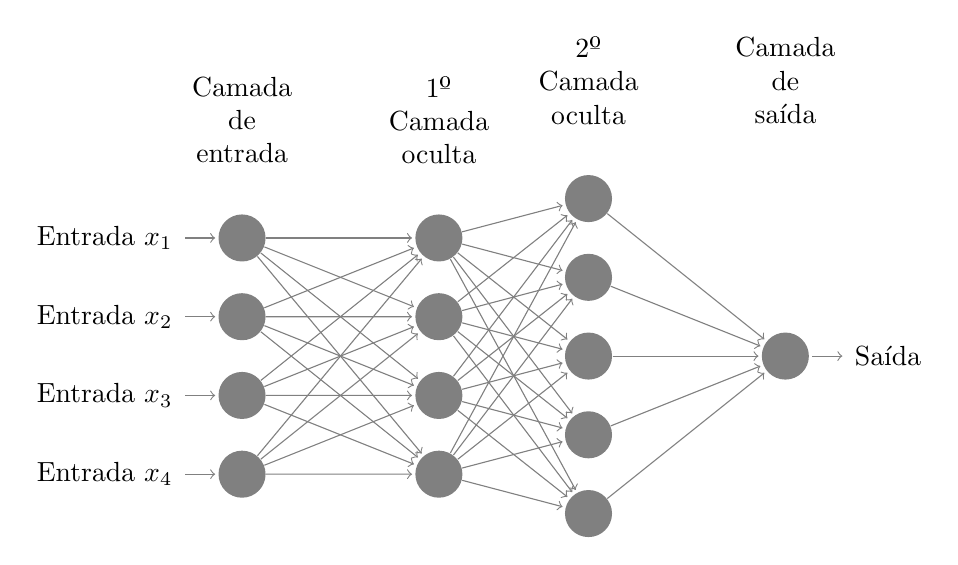
\begin{tikzpicture}[shorten >=1pt,->,draw=black!50, node distance=\layersep]
    \tikzstyle{every pin edge}=[<-,shorten <=1pt]
    \tikzstyle{neuron}=[circle,fill=black!25,minimum size=17pt,inner sep=0pt]
    \tikzstyle{input neuron}=[neuron, fill=black!50];
    \tikzstyle{output neuron}=[neuron, fill=black!50];
    \tikzstyle{hidden neuron}=[neuron, fill=black!50];
    \tikzstyle{annot} = [text width=4em, text centered]

    % Draw the input layer nodes
    \foreach \name / \y in {1,...,4}
    % This is the same as writing \foreach \name / \y in {1/1,2/2,3/3,4/4}
        \node[input neuron, pin=left:Entrada $x$$_\y$] (I-\name) at (0,-\y) {};

    % Draw the hidden layer nodes
    \foreach \name / \y in {1,...,4}
        \path[yshift=0cm]
            node[hidden neuron] (H-\name) at (\layersep,-\y cm) {};
            
    % Draw the second hidden layer nodes
    \foreach \name / \y in {1,...,5}
        \path[yshift=0.5cm, xshift=1.9cm ]
            node[hidden neuron] (J-\name) at (\layersep,-\y cm) {};

    % Draw the output layer node
    \node[output neuron,pin={[pin edge={->}]right:Saída}, right of=J-3] (O) {};

    % Connect every node in the input layer with every node in the
    % hidden layer.
    \foreach \source in {1,...,4}
        \foreach \dest in {1,...,4}
            \path (I-\source) edge (H-\dest);
   
   % Connect every node in the hidden layer 1 with every node in the
    % hidden layer 2.     
     \foreach \source in {1,...,4}
        \foreach \dest in {1,...,5}
            \path (H-\source) edge (J-\dest);

    % Connect every node in the hidden layer with the output layer
    \foreach \source in {1,...,5}
        \path (J-\source) edge (O);

    % Annotate the layers
    \node[annot,above of=H-1, node distance=1.5cm] (hl) {1º Camada \\ oculta};
    \node[annot,above of=J-1, node distance=1.5cm] (hl2) {2º Camada \\ oculta};
    \node[annot,left of=hl] {Camada de entrada};
    \node[annot,right of=hl2] {Camada de \\ saída};
    %\node[annot,above of=H-1, node distance=1.5cm] (hl) {Camada de \\ Saída};
\end{tikzpicture}
    \caption{Rede de múltiplas camadas}
    \fonte{Adaptado de \citeonline{livroNunes2016}}
    \label{figure:multilayer_perc}
\end{figure}

Por fim as redes recorrentes, que recebem este nome por conta da realimentação entre os neurônios da mesma camada, ou seja, a saída de um neurônio em uma camada, pode servir como entrada para outro neurônio da mesma camada \cite{Nelson2017}.

Estas formas de organização presentes nas arquiteturas, estão intimamente relacionadas ao processo de aprendizado que é aplicado nas RNAs \cite{Haykin2001}.

\subsection{Processo de aprendizado}

Um dos pontos mais relevantes das RNAs é a generalização \cite{livroNunes2016}, onde treina-se levando em consideração um conjunto amostral \textit{A}, este que faz uma boa representação do problema resolvido na tarefa (REF), e então após este processo a rede consegue realizar a tarefa não somente para o conjunto \textit{A}, mas também para um conjunto \textit{C} qualquer \cite{livroNunes2016}.

Porém para a generalização, como citado, é necessário um processo de treinamento, este que seja adequado a arquitetura de rede neural. \citeonline{livroNunes2016} definem processo de treinamento como um algoritmo que, através de seus passos bem definidos ajusta os pesos sinápticos da rede com o objetivo de permitir o mapeamento das relações dos dados e então realizar o processo de generalização. 

Os processos de treinamento podem adotar diferentes estratégias para ensinar as RNAs, e cada estratégia gera um algorítimo de aprendizado diferente, sendo os principais, os algorítimos de aprendizado supervisionado e não-supervisionado.

No aprendizado supervisionado, há rótulos $y^{(t)}$ que indicam o comportamento $\widehat{y}$ que a rede deve apresentar para cada $x^{(t)}$ presente em um conjunto de dados $\{(x^{(t)}, y^{(t)}): 1 \leqslant t \leqslant T\}$ \cite{bezerra2016}. Desta forma, de acordo com os resultados apresentados, ajustes são feitos nos pesos sinápticos e limiares dos neurônios da rede \cite{livroNunes2016}, com o objetivo de fazer com que a saída da rede seja o mais próximo possível de $y^{(t)}$ \cite{Osorio1999}. Já o aprendizado não supervisionado, são utilizados apenas os dados, sem qualquer tipo de rótulo e sua intenção é realizar agrupamentos \cite{Camila2017}, levando em consideração características relevantes, estas identificadas pela rede.

% No aprendizado supervisionado, é considerado adisponibilidade de um conjunto de treinamento  é o vetor de características que está associado ao componente $y^{t}$ \cite{bezerra2016}, e então, para cada $x^{t}$ a rede gera um componente resultante $\widehat{y}$, este que será utilizado  

% NG -> Neste caso é o curso do Andrew NG
% No aprendizado supervisionado, o usuário indica o comportamento que a RNA deve apresentar dado um conjunto de dados qualquer, desta forma, a RNA pode ir ajustando os pesos sinápticos de seus neurônios com o objetivo de produzir o mesmo resultado apresentado pelo usuário. Já o aprendizado não supervisionado, oposto do supervisionado, é apresentado para a RNA apenas o conjunto de dados, e a RNA se encarrega de aprender sobre aquele conjunto de dados. Este tipo de aprendizado pode ser utilizado para deixar a RNA identificar os padrões presentes nos dados, e tirar informações destes padrões (NG, 2013). 

% \subsubsection{Transferência de aprendizado}
% Isto aqui está completamente sem sentido nesta parte... (25/02/2019)

% Buscar referências para a primeira afirmação feita (25/02/2019)
% Certos tipos de arquiteturas de RNAs são formadas por dezenas ou mesmo centenas de neurônios, e isto exige grandes conjuntos de dados em seu treinamento, grande poder computacional e tempo \cite{Carneiro2017, decio2017} para possibilitar a generalização do algoritmo, porém comumente para boa parte dos problemas há apenas pequenos conjuntos de dados \cite{Ponti2018} e nem sempre há capacidade computacional para a realização dos treinamentos, para estes casos, pode-se empregar as técnicas de Transferência de aprendizado.

% Estou com dúvida se deixo este sub-tópico aqui....Ele faz bem mais sentido no tópico de aprendizado profundo

% Um dos grandes desafios em certas arquiteturas de RNAs, que dispõem de milhares de parâmetros a serem ajustados durante o processo de treinamento, utilizar o conhecimento adquirido no contexto de uma tarefa, e utiliza-lo em um contexto diferente do original...

% Em certas arquiteturas de RNAs, que possuem grandes quantidades de parâmetros a serem ajustados, 

% Em certas arquiteturas de RNAs, que possuem grandes quantidades de parâmetros a serem ajustados, 

% Em aprendizado profundo existe a necessidade de datasets com centenas de milhares de imagens...
% \par Explicar sobre transferência de aprendizado

\section{Aprendizado Profundo}

O Aprendizado Profundo (AP) apresenta uma abordagem diferente para os problemas resolvidos com técnicas de RNA, onde múltiplas camadas são empregadas nas arquiteturas, permitindo assim que problemas mais complexos e sofisticados sejam mapeadas \cite{Goodfellow-et-al-2016}.

As características dos algoritmos de AP fizeram com que estes chegassem ao estado da arte em diversos casos, como em \cite{Shankar2017} e \cite{Krizhevsky2012}. 

% Goodfellow realmente falou insto ? (25/02/2019)
% O Aprendizado profundo (AP) apresenta uma abordagem diferente para os problemas resolvidos com técnicas de RNA, porém, no caso de AP, muitas camadas são empregadas (GOODFELLOW, 2016) nas arquiteturas das redes neurais (Figura 5).

% Imagem colorida de mais...Possivelmente montar a estrutura com as figuras do Felipe Carvalho (25/02/2019)
%\image{0.6}{snn_vs_dl.png}{Diferenças entre redes neurais simples e Deep Learning}{ml_vs_dl}

% Shankar ? (25/02/2019)
% A utilização de múltiplas camadas, cada um com dezenas de neurônios, permitiu as técnicas de DL chegarem ao estado-da-arte em muitos problemas que envolvem o AM (SHANKAR, 2017).  Além disto, de acordo com Andrew NG, o processo de aprendizado destas redes melhora muito com o aumento dos dados (Figura 6), diferente do que ocorria com arquiteturas e algoritimos de aprendizado de máquinas antigos.

% Imagem escura de mais....Criar um plot talvez, algo para deixar bonito msm... (25/02/2019)
% \image{0.4}{dl_vs_dados.png}{Deep Learning X Quantidade de dados}{dl_vs_dados}

% De acordo com (Andres, ????) -> Faltou inserir o ano aqui (25/02/2019)
% Ainda de acordo com Andrew, isto ocorre pois ao utilizar múltiplas camadas, diversos recursos são captados dos dados, fazendo com que o processo de aprendizado se torne eficaz, e tende a melhorar ainda mais com o aumento da quantidade de dados utilizados no processo de treinamento. 

% A utilização de múltiplas camadas, permitiram que diferentes técnicas pudessem ser utilizadas dentro de uma rede neural, e isto fez com que diversas arquiteturas, para os mais variados fins fossem criados.

\subsection{Redes Neurais Convolucionais}

Redes Neurais Convolucionais (do inglês \textit{Convolutional Neural Network} - CNN) são uma variação das redes MLP, tendo sua criação inspirada no processo biológico de processamento de dados visuais \cite{Caroline2016}. Estas arquiteturas de AP, são capazes de subdividir os dados para tentar extrair características relevantes a classificação, reduzindo assim o números de parâmetros que deverão ser ajustados pela rede \cite{Miyazaki2017}, assim, melhorando o processo de treinamento \cite{Miyazaki2017}. % Verificar o ARAUJO, 2017 -> Para inserir nesta parte

As CNNs são utilizadas principalmente em dados com estruturas de grade, como por exemplo, processamento de fala e entendimento da linguagem natural (Uma dimensão, convolução temporal) \cite{Miyazaki2017} e segmentação e classificação de imagens (Duas dimensões, convolução espacial) \cite{Miyazaki2017, Goodfellow-et-al-2016}.

Um dos primeiros modelos de CNNs propostos foi a LeNet \cite{LeCun1998} (Figura \ref{figure:lecun_basic}), esta que é formada por uma sequência de camadas onde cada uma delas possui uma função específica \cite{Carneiro2017}. 

% Colocar esta descrição...
% Estrutura básica de CNN proposta por LeCun aplicada na identificação de célcular normais e anormais....
\image{0.6}{cnn_lenet.JPG}{Estrutura básica de CNN proposta por LeCun, 1998}{figure:lecun_basic}{\citeonline{Carneiro2017}}

As três camadas fundamentais para uma CNN, apresentadas por \citeonline{LeCun1998}, e ilustradas na Figura TTY, são as seguintes: convolucional, de \textit{pooling} e totalmente conectada.

% SAVARESE, 2018 -> https://web.stanford.edu/class/cs231a/lectures/intro_cnn.pdf
% ARAÚJO, 2017 -> Redes neurais convolucionais com tensorflow: Teoria e Prática 
% É legal colocar: `do inglês...` ? (25/02/2019)
% Redes neurais convolucionais, do inglês, \textit{Convolutional Neural Network} são um tipo de rede neural profunda, especializadas em análise de elementos visuais, tais como imagens e vídeos (SAVARESE, 2018).  Sua especialidade em dados visuais permitiu um grande avanço nas áreas de visão computacional, especialmente por estas serem mais fáceis de treinar, quando comparado a redes neurais comuns em trabalhos com imagens (ARAÚJO, 2017).

% Um dos primeiros modelos de CNN propostos foi a LeNet-5 (LECUN et al, 1998), proposta por Yann LeCunn em 1998, e mesmo evoluindo, os conceitos apresentados por LeCun continuam sendo aplicados. Nesta arquitetura, uma sequência de camadas convolucionais, de \textit{pooling} e totalmente conectadas são utilizadas (ARAÚJO, 2017).

% As camadas convolucionais, que são a grande diferença das CNN para outros tipos de RNA, trabalham como filtros, recuperando apenas pontos importantes da imagem para a classificação, isto através de uma matriz de pesos que é utilizada nas convoluções (ARAÚJO, 2017). Após o filtro realizado por esta camada, as imagens resultantes do filtro são passadas para a camada de \textit{pooling}, estas camadas que básicamente reduzem a dimensionalidade das resultantes. Por fim, as camadas totalmente conectadas são as responsáveis em realizar a multiplicação ponto a ponto dos sinais recebidos (imagens) e aplicar uma função de ativação, que produzirá a probabilidade de cada uma das classes esperadas na classificação (ARAÚJO, 2017).

% A Figura 7 demonstra a arquitetura de LeCun sendo utilizada para a classificação de imagens de tumores, podendo ter como resultado às classes \textbf{normal} ou \textbf{anormal}.

% Modelo proposto por LeCun 98 (LeNet-5), aplicado a identificação de anomalias....
% \image{0.6}{cnn_lenet.JPG}{Estrutura básica de CNN proposta por LeCun, 1998}{lecun_basic}

% Veja que, o diferencial citado acima, na utilização das convoluções está justamente na quantidade de elementos que são utilizados para a classificação, em RNA comuns, ao realizar a classificação de imagens, deve-se ter de neurônios na RNA a mesma quantidade de píxels presentes na imagem a ser classificada, o que nas CNN não ocorre, exatamente por conta dos filtros que são criados (PONTI, 2017). 

\subsubsection{Camada convolucional}

As camadas convolucional (do inglês \textit{Convolutional layer} - CL) são conjuntos de filtros não lineares que percorrerem os dados de entrada sequencialmente e produzem os mapas de características \cite{Miyazaki2017}. O processo de percorrer os dados de entrada ocorrer através de passos (\textit{strides}), podendo passar de \textit{pixel} em \textit{pixel} no caso de imagens ou mesmo de posição em posição da matriz de entrada.

A Figura \ref{figure:conv_complete} demonstra o processo de convolução, nesta, um filtro 3x3 passa sobre uma região dos dados, com passo igual a um, e a multiplicação entre eles é realizada, e os valores resultantes são somados e colocados no mapa de características.

% Especificar a fonte...
% Adaptada de: https://www.vaetas.cz/posts/intro-convolutional-neural-networks/
\image{0.6}{conv_completa.png}{Processo de convolução}{figure:conv_complete}{Adaptado de https://www.vaetas.cz/posts/intro-convolutional-neural-networks/}

\subsubsection{Camada de Pooling}

% Buscar referências...
A camada de \textit{Pooling}, comumente utilizada após uma certa camada de convolução \cite{Caroline2016}. Sua função é reduzir a dimensionalidade dos dados do mapa de características \cite{Caroline2016}. Esta redução é realizada principalmente para agilizar o processo de treinamento \cite{Caroline2016}.

Esta diminuição é feita através do agrupamento de valores, este que através de uma janela MxN, aplica-se uma função, normalmente uma função de média ou de valor máximo \cite{Amidi2018}.

A Figura \ref{figure:pooling} apresenta uma operação de \textit{Pooling} feita através de um filtro 2x2, com a função de valor máximo.

% Figura de 
\image{0.6}{pooling.png}{Processo de \textit{Pooling}}{figure:pooling}{Adaptado de \citeonline{rawat2017}}

\subsubsection{Camada totalmente conectada}

A saída das camadas convolucionais e de \textit{Pooling} geram as características extraídas dos dados de entrada \cite{Carneiro2017}. As camadas totalmente conectadas utilizam estas características para classificar os dados. Estas camadas representam uma RNA convencional, uma MLP \cite{Haykin2001}, dentro desta RNA, sua última camada contém uma função de ativação, normalmente \textit{softmax}, responsável pela classificação final dos resultados \cite{Bishop2006}. 

\subsubsection{Transferência de Aprendizado}

Realizar treinamentos de CNNs requer grandes quantidades de dados, não sendo comum realizar treinamento deste tipo de rede do zero \cite{Carneiro2017}, isto porque mesmo havendo uma melhora nos parâmetros que precisam ser ajustados com a aplicação dos filtros de convolução, normalmente estas redes apresentam muitas camadas, e realizar o ajuste de cada camada pode exigir muitos dados. Desta forma é comum utilizar modelos que já possuem parâmetros ajustados para outros conjuntos de dados \cite{Ponti2018}, ou seja, aplica-se um domínio geral em um domínio específico, e este processo é nomeado de Transferência de aprendizado.

De acordo com \citeonline{Ponti2018} existem diversas abordagens para a realização da transferência de aprendizado, sendo alguns deles: (i) Permitir que o algoritmo de treino ajuste todos os pesos presentes na rede com os novos dados, (ii) Congelar algumas camadas e assim limitar o número de parâmetros treinados pela rede, (iii) Adicionar mais camadas no modelo e realizar o treinamento somente destas novas camadas.

A escolha da abordagem de transferência pode variar de acordo com a similaridade do novo conjunto de dados em relação ao antigo e também a seu tamanho \cite{Carneiro2017}.

% \subsection{Camada totalmente conectada} % Esta seção fica aqui pois faz parte das redes neurais convolucionais (02/02/2019), (03/02/2019) R: não! Isto faz parte de rede neural mesmo! 

\subsection{Mobilenet}

MobileNet é um modelo de CNN criado para apresentar bons resultados em classificações de imagens e ao mesmo tempo, ser leve, tanto no tamanho em memória, quanto em suas operações. Faz isto através da aplicação de técnicas de convolução profunda separável (do inglês \textit{Depthwise Separable Convolution}), este que basicamente aplica um filtro para cada camada de cor, permitindo assim que o modelo seja utilizado em sistemas \textit{web} e aplicativos de \textit{Smartphones} \cite{howard2017mobilenets}.

\subsection{Posenet}

\par Posenet é um modelo de CNN, criado com base nos trabalhos \cite{george2017} e \cite{george2018} que realiza a identificação de 17 pontos do corpo humano (Figura \ref{figure:posenet_poses}), de um ou vários usuários. Este modelo que, por ser leve, pode ser aplicado nos mesmos contextos que o Mobilenet.

\image{0.6}{posenet_poses_original.png}{Pontos identificados pelo Posenet}{figure:posenet_poses}{Adaptado de https://medium.com/tensorflow/real-time-human-pose-estimation-in-the-browser-with-tensorflow-js-7dd0bc881cd5}

\section{Tecnologias}

Esta seção demonstra as tecnologias utilizadas durante a implementação do presente trabalho.

\subsection{Keras}

Keras é um biblioteca de Python, que permite a criação em alto nível de redes neurais artificiais, além de disponibilizar funcionalidades para a aplicação de transferência de aprendizado em modelos já treinados, presentes na biblioteca. Os códigos são escritos com Keras, e podem ser executados com as seguintes bibliotecas \textit{TensorFlow}, \textit{Microsoft Cognitive Toolkit} (CNTK) e \textit{Theano} \cite{chollet2015}.

\subsection{TensorFlow.js}

TensorFlow.js (TFJS) é uma biblioteca JavaScript desenvolvida para criar e executar algoritmos de aprendizado de máquina. Os modelos desenvolvidos com TFJS, podem ser executados em um navegador \cite{tensorflowjs2019}. Esta é uma biblioteca que faz parte do ecossistema TensorFlow, criado pelo Google, assim, os modelos criados em outros ambientes do ecossistema, como por exemplo em Python, podem ser facilmente portados para o TFJS \cite{tensorflowjs2019}.

\subsection{Google Colaboratory}

Colaboratory (Colab) é uma ferramenta criada pelo Google, que permite a fácil execução de algorítimos de aprendizado de máquina. Colab é criado sobre o pacote Jupyter, um ambiente interativo, executado no navegador, que permite a execução de linguagens interpretadas \cite{PER-GRA:2007}. Todo o ambiente do Colab é executado sobre máquinas aceleradas por GPU, o que diminui o tempo de execução de processos de treinamento de modelos.
